\chapter{Implementation}\label{implementation}

\section{Persistenz}
\subsection{Auswahl Persistenz-Provider}
Bereits zu Beginn stellte sich die Frage, warum man welche der drei m\"oglichen und im Abschnitt ``\ref{grundlagen:persistenz} \titleref{grundlagen:persistenz}'' aufgelisteten Persistenz-Provider Mapper, Record oder ScalaJPA  verwenden sollte.

Ich versuchte herauszufinden und auszuf\"uhren, wie weit Ans\"atze hinsichtlich Dokumentation, aktive Weiterentwicklung und Reifegrad der Implementation sind.

\subsubsection{Aktive Weiterentwicklung}
Ein Blick auf die verschiedenen Commit Histories der Persistenz Module Mapper\footnote{http://github.com/lift/lift/commits/master/framework/lift-persistence/lift-mapper} und Record\footnote{http://github.com/lift/lift/commits/master/framework/lift-persistence/lift-record} zeigt schnell auf, dass in beiden Frameworks aktiv nicht sonderlich viel geschieht. \"Anderungen im Bereich der Persistenz-Libraries finden momentan vorallem im Bereich der NoSQL Datenbanken statt. 

\subsubsection{Dokumentation}
W\"ahrend die Dokumentation von Mapper\footnote{http://www.assembla.com/wiki/show/liftweb/Mapper} noch einigermassen anspricht, kann man zum Mapping mit dem Record Framework ausser ganz wenige Beispiele in \cite[p. 79 - 113]{chen2009lift} nicht viel auffinden.

\subsubsection{Reifegrad}
Der Reifegrad der im Lift Framework enthaltenen Persistenz-Bibliotheken ist meines Erachtens gering. Anforderungen wie das Mappen von Hierarchien (Beispiele in Hibernate Table per Klasse, Table per Hierarchie) fehlen g\"anzlich. Die Relationen zwischen den Klassen sind relativ unflexibel und gen\"ugen h\"ochstens, wenn man ein Projekt auf der ``Gr\"unen Wiese'' starten kann. Der dritte wichtige Mangel ist, dass mit der Verwendung von Mapper und Record eine Kopplung der gesamten Applikation ans Persistenz-Framework passiert. Siehe dazu Abschnitt ``\ref{persistenz:kopplung} \titleref{persistenz:kopplung}''.


\subsubsection{Fazit}
Meines Erachtens liefern Mapper und Record nicht das, was wir uns von bereits existierenden Frameworks wie Hibernate gewohnt sind. Ich habe mich aus oben beschriebenen Gr\"unden dazu entschieden, JPA 2.0 und Hibernate in der Version 3.5.1 im Persistenz-Layer zu verwenden. 

\subsection{Domain Mapping}
Ich habe die Mappings der Dom\"anenklassen mittels im Abschnitt ``\ref{grundlagen:integration:java} \titleref{grundlagen:integration:java}'' kurz angesprochenen Annotationen gemacht. Ich gehe im folgenden auf das Mapping der User Klasse ein, werde aber an dieser Stelle auf die Beschreibung der Mappings aller Klassen verzichten. 

\subsubsection{Klasse User}
Die Mapping Informationen f\"ur Hibernate respektive JPA befinden sich in Klasse ch.plannr.model.User. Die Klasse verwendet als Mixins folgende Traits:
\begin{itemize}
	\item \textbf{MegaBasicUser - } verf\"ugt in Anlehnung an MegaProtoUser\footnote{Mega ProtoUser ist die Basis-User-Klasse f\"ur das Mapper Framework und stellt eine Basis f\"ur die Benutzerverwaltung zur Verf\"ugung} \"uber die Funktionalit\"aten, die im Zusammenhang mit der Registrierung, Login, Passwort-Reset ben\"otigt werden. 
	\item \textbf{Domain -} definiert abstrakte Methoden zur Umwandlung von Objekten in XML und in die JSON\footnote{Javascript Object Notation}. 
	\item \textbf{Persistent - }Stellt in Anlehnung an das Active Record Design Pattern Methoden zum Persistieren, L\"oschen, Editieren von Objekten zur Verf\"ugung.	
\end{itemize}

Zu persistierende Objekte werden als Entities bezeichnet und m\"ussen in JPA mit 
\begin{lstlisting}[caption=User: ScalaJPA Entity Definiton]
@Entity
@Table(name = "TBL_USER")
\end{lstlisting}

annotiert werden. Mit Table kann man den Tabellennamen spezifizieren. Was auch ein Mapping auf Legacy Datenbanken erm\"oglichen w\"urde.

Die Id des Benutzers kann bei bestimmten Datenbanken automatisch ermittelt werden. In meinem Fall MySQL wird das mittels 
\begin{lstlisting}[caption=User: ScalaJPA Id mit Auto-Increment]
@Id
//@GeneratedValue(
//	strategy = GenerationType.SEQUENCE, 
//	generator="user_seq")
@GeneratedValue(strategy = GenerationType.AUTO)
@Column(name = "ID")
var id: Long = _
\end{lstlisting}
gemappt. Im Fall von Oracle m\"usste der GenerationType.SEQUENCE verwendet werden.
Normale Properties ben\"otigen eigentlich keine Annotation mehr, per Default werden in JPA alle Properties als Spalten angelegt, mit der @Column Annotation kann man allerdings die Defaults (Constraints, Spaltenname) \"uberschreiben. @NotNull und @NotEmpty sind Annotationen zur Validierung von Objekten (siehe Abschnitt ``\ref{jpa:validation} \titleref{jpa:validation}''). Die Annotation @BeanProperty sorg daf\"ur, dass f\"ur ein Feld Getter- und Setter-Methoden erstellt werden. Dies ist vorallem zur Interoperabilit\"at mit Java-Frameworks teilweise m\"oglich - in diesem Fall wird es ebenfalls f\"ur die Validierung ben\"otigt. 
\begin{lstlisting}[caption=User: ScalaJPA firstname Mapping]
@Column(name = "FIRST_NAME", nullable = false)
@NotNull
@NotEmpty
@BeanProperty
var firstname: String = _
\end{lstlisting}

Des weiteren sind die Annotationen @Embedded\footnote{@Embedded bietet die M\"oglichkeit, Attribute zwar in der selben Tabelle (embedded) zu speichern, allerdings im Objekt-Orientierten Modell in ein andere Instanz wie zum Beispiel in ein Adress-Objekt abzurufen} und die verschiedenen Beziehungen zu anderen Tabellen @ManyToOne, @OneToMany und @ManyToMany\footnote{Mittels @ManyToOne, @OneToMany, @ManyToMany k\"onnen uni- und bidirektionale Beziehungen realisiert werden.} interessant. 



\subsection{Validation}\label{jpa:validation}
Annotationen wie @NotNull, @Null, @Past, @Future sind definiert \"uber den JSR330 (Bean Validation 1.0). Mittels Bean Validation lassen sich Validierungen auf allen Ebenen des Systems durchf\"uhren. Zum Beispiel lassen sich User-Objekte bereits ohne Speicherung validieren und entsprechend f\"ur jedes Property Fehlermeldungen in der View bereitstellen. Auf der Ebene der Datenbank k\"onnen automatisch Constraints anhand dieser annotierten Properties setzen.

Alle Dom\"anenklassen die als Mixin Persistent[T] verwenden k\"onnen mittels der methode validate validiert werden. Die Validierung wird vollumf\"anglich anhand der in den Klassen enthaltenen Annotationen gemacht. Als R\"uckgabewert werden die Constraints-Verletzungen innerhal eines Sets zur\"uckgeliefert. Ich verwende diese Constraints-Verletzungen weiter f\"ur die Anzeige in der View. Zum Beispiel der Validierung bei der Registrierung werden bei unvollst\"andiger Eingabe folgende Fehler angezeigt:
 \begin{figure}
  	\centering
    	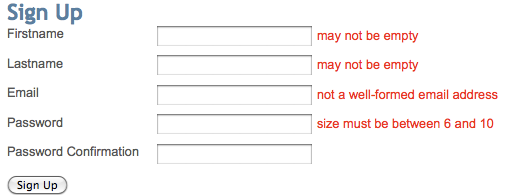
\includegraphics[width=12cm]{images/validation_registration}
        	\caption{Formular Validierung: Registration}
\end{figure}


Die Implementation der Methode validate ist relativ einfach und sieht folgendermassen aus:
\begin{lstlisting}[caption=Validation innerhalb von ch.plannr.common.persistence.Persistence]
@Transient
private val validatorFactory = 
		Validation.buildDefaultValidatorFactory();

@Transient
private val validator = validatorFactory.getValidator();
  
def validate() = {
  validator.validate(this)
}
\end{lstlisting}

\subsection{Aufbau des Domain Modells}
\section{Security: Registrierung, Login}
\section{Navigation}
\section{Mail-Versand (Notifikationen)}
\section{Evaluation Kalender}



\chapter{Deployment}
\section{Setup von Entwicklungs-, Test- und Produktiv-Umgebung}





